
\section{| 3 Regularized Linear Regression}

\subsection{| 3.1 Visualizing the dataset}

\begin{figure}[H]
    \centering
    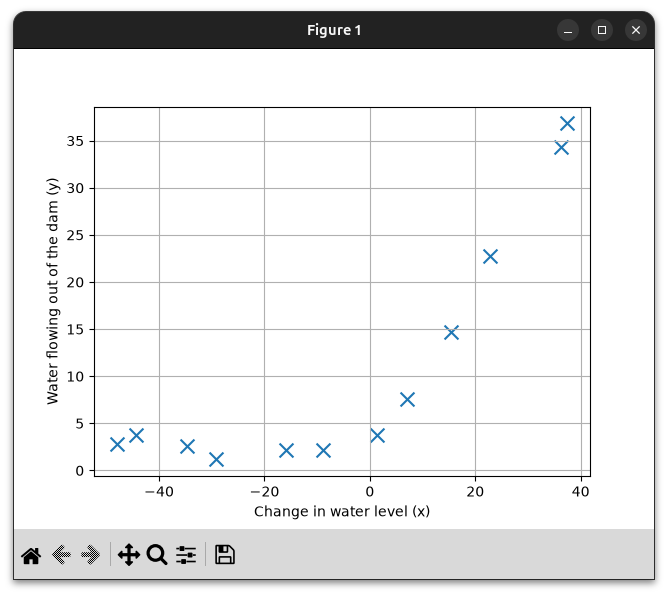
\includegraphics[width=0.75\linewidth]{figure/image.png}
    \label{fig:placeholder}
\end{figure}

\begin{figure}[H]
    \centering
    
\includegraphics[width=0.75\linewidth]{figure/image1.png}
    \label{fig:placeholder}
\end{figure}


\subsection{| 3.2 Regularized linear regression cost function}

\begin{lstlisting}
import numpy as np

def linearRegCostFunction(X, y, theta, Lambda):
    """computes the cost of using theta as the parameter for linear regression
    to fit the data points in X and y.
    Returns the cost in J
    """

    # Initialize some useful values

    m,n = X.shape # number of training examples
    theta = theta.reshape((n,1)) # in case where theta is a vector (n,) 
    J = 0.

    # ====================== YOUR CODE HERE ======================
    # Instructions: Compute the cost of regularized linear
    #               regression for a particular choice of theta.
    #
    #               You should set J to the cost.
    #

    h = X @ theta
    e = h - y.reshape((m,1))

    J_error = np.sum(e**2) / (2*m)
    J_reg = (Lambda / (2*m)) * np.sum(theta[1:]**2)
    J = J_error + J_reg

    # ==================================================
    return J.flatten()
\end{lstlisting}

\begin{figure}[H]
    \centering
    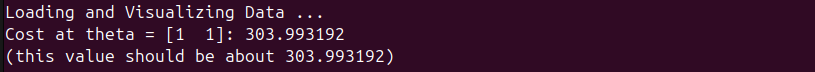
\includegraphics[width=0.75\linewidth]{figure/image2.png}
    \label{fig:placeholder}
\end{figure}


\subsection{| 3.3 Regularized linear regression gradient}

\begin{lstlisting}
import numpy as np

def linearRegGradientFunction(X, y, theta, Lambda):
    """computes the gardients of the cost using theta as the parameter for linear regression
        to fit the data points in X and y.
        Returns the gradient in grad
     """

    # Initialize some values
    m,n = X.shape # number of training examples
    theta = theta.reshape((n,1)) # in case where theta is a vector (n,)
    grad = 0.

    # ====================== YOUR CODE HERE ======================
    # Instructions: Compute the gradient of regularized linear
    #               regression for a particular choice of theta.
    #
    #               You should set grad to the gradient.
    #

    h = X @ theta
    e = h - y.reshape((m,1))

    grad = (X.T @ e) / m
    grad[1:] += (Lambda / m) * theta[1:]

    # ==================================================
    return grad.flatten()
\end{lstlisting}

\begin{figure}[H]
    \centering
    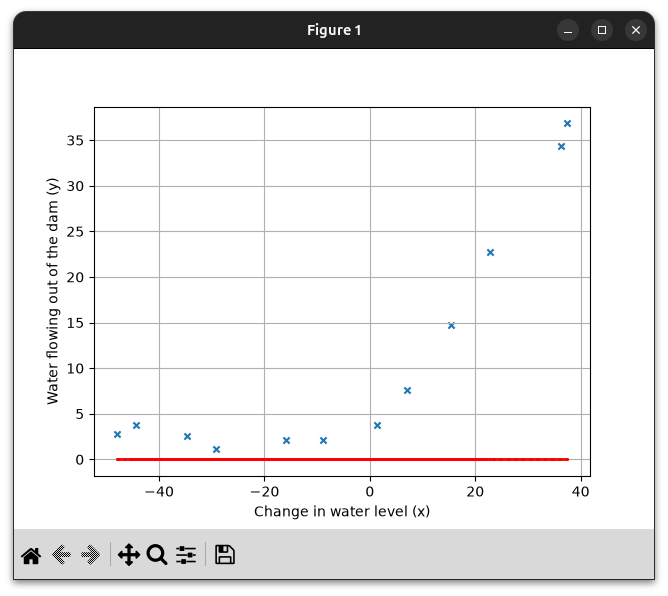
\includegraphics[width=0.75\linewidth]{figure/image3.png}
    \label{fig:placeholder}
\end{figure}

\begin{figure}[H]
    \centering
    
\includegraphics[width=0.75\linewidth]{figure/image4.png}
    \label{fig:placeholder}
\end{figure}

\subsection{| 3.4 Fitting linear regression}


\begin{lstlisting}
from unittest import result

import numpy as np
from scipy.optimize import minimize

from linearRegCostFunction import linearRegCostFunction
from linearRegGradientFunction import linearRegGradientFunction


def trainLinearReg(X, y, Lambda, Xval=None, yval=None, maxiter=200):

    """trains linear regression using
    the dataset (X, y) and regularization parameter lambda. Returns the
    trained parameters theta.
    """

    # Initialize Theta and costs history
    theta = np.zeros(X.shape[1])
    n = theta.size  # number of parameters
    cost_train = []
    cost_val = []

    # fonction permettant a minimize de recuperer l'evolution des thetas
    thetas = []
    def save_step(*args):
        for arg in args:
            if type(arg) is np.ndarray:
                thetas.append(arg)

    # Initialize Theta
    initial_theta = np.zeros((X.shape[1]))

    # Create "short hand" for the cost function to be minimized
    costFunction = lambda t: linearRegCostFunction(X, y, t, Lambda)
    gradFunction = lambda t: linearRegGradientFunction(X, y, t, Lambda)

    # Descente de gradient
    result = minimize(costFunction, initial_theta, method='CG', jac=gradFunction, options={'disp': False, 'maxiter': maxiter, 'return_all':True}, callback=save_step)


    # ====================== YOUR CODE HERE ======================
    # Instructions: Compute
    #   - theta the final thetas
    #   - the training cost vs iteration number from thetas
    #   - the validation cost vs iteration number from thetas

    # outputs
    theta = result.x

    for t in thetas:
        cost_train.append(linearRegCostFunction(X, y, t, 0)[0])

    if Xval is not None and yval is not None:
        for t in thetas:
            cost_val.append(linearRegCostFunction(Xval, yval, t, 0)[0])

    # ==================================================

    # force to np array
    cost_train = np.array(cost_train)
    cost_val = np.array(cost_val)

    return theta, cost_train, cost_val
\end{lstlisting}

\begin{figure}[H]
    \centering
    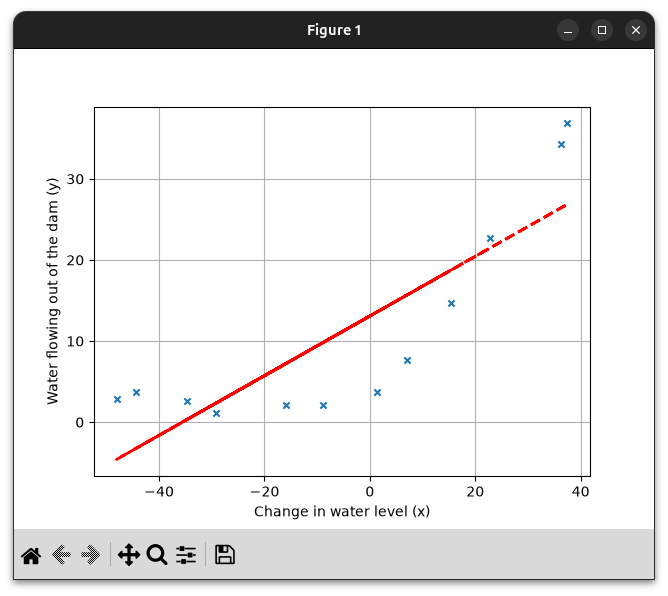
\includegraphics[width=0.75\linewidth]{figure/image5.png}
    \label{fig:placeholder}
\end{figure}

The training was successful, and the algorithm found the optimal parameters \(\theta_0\) and \(\theta_1\) that minimize the cost function.

However, the fitted line does not follow the data points well, especially at the extremes, where the data shows a nonlinear behavior.

This indicates underfitting (high bias) because the linear regression model is too simple to represent the data accurately.


\section{| 4 Bias-variance}

\subsection{| 4.1 Learning curves}

\begin{lstlisting}
import matplotlib.pyplot as plt
from trainLinearReg import trainLinearReg

from trainLinearReg import trainLinearReg
from linearRegCostFunction import linearRegCostFunction
from linearRegGradientFunction import linearRegGradientFunction

def learningCurve(X, y, Lambda, Xval, yval, ax=plt.gca(), maxiter=2000):
    """returns the train and validation/test set costs for a learning curve. In particular,
    it returns two vectors of the same length - cost_train and
    cost_val.

    In this function, you will compute the train and validation costs.
    """

    # Number of training examples
    m, _ = X.shape
    cost_train = 0.
    cost_val = 0.

    # ====================== YOUR CODE HERE ======================
    # Instructions: Fill in this function to return training costs in
    #               cost_train and the validation errors in cost_val.
    #

    # Erreur d'apprentissage et de generalisation
    _, cost_train, cost_val = trainLinearReg(X, y, Lambda, Xval, yval, maxiter)

    # ==============================================

    # display
    plt.figure()
    ax.plot(range(cost_train.size), cost_train, color='b', lw=2, label='Train')
    ax.plot(range(cost_val.size), cost_val, color='r', lw=2, label='Validation')
    ax.set_title('Learning curves for linear regression')
    ax.grid()
    ax.set_xlabel('Number of iterations')
    ax.set_ylabel('Cost')
    ax.legend(loc='upper right', shadow=True, fontsize='x-large', numpoints=1)

    return cost_train, cost_val
\end{lstlisting}

\begin{figure}[H]
    \centering
    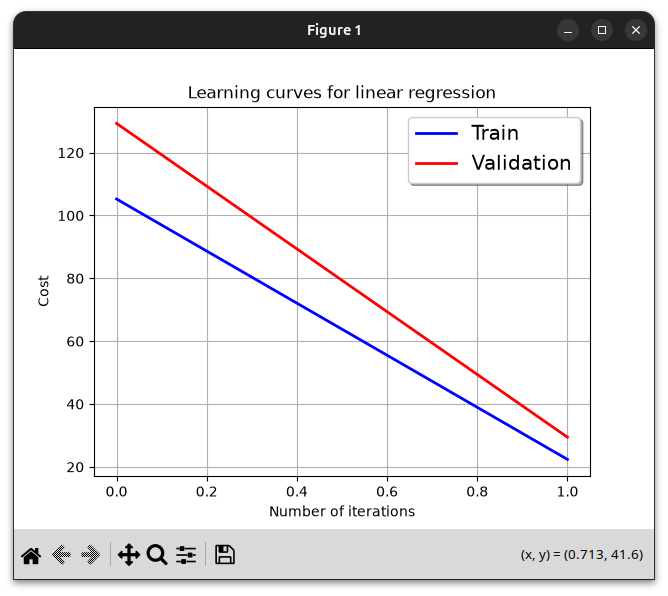
\includegraphics[width=0.75\linewidth]{figure/image6.png}
    \label{fig:placeholder}
\end{figure}

Both training and validation costs decrease during training, showing that the model is learning.

However, both costs remain relatively high and close to each other.

This indicates underfitting (high bias) because the linear model is too simple to fit the data well.

\section{| 5 Polynomial regression}



\begin{lstlisting}
import numpy as np

def polyFeatures(X, p):
    """takes a data matrix X (size m x 1) and
    maps each example into its polynomial features where
    [X X**2 X**3 ...  X**p]
    """
    # You need to return the following variables correctly.
    X_poly = np.zeros((X.shape[0], p))

    # ====================== YOUR CODE HERE ======================
    # Instructions: Given a vector X, return a matrix X_poly where the p-th 
    #               column of X contains the values of X to the p-th power.
    #
    # 

    for i in range(p):
        X_poly[:, i] = X[:, 0] ** (i + 1)
    
    # =============================================
    return X_poly

\end{lstlisting}



\subsection{| 5.1 Learning Polynomial Regression}

\begin{figure}[H]
    \centering
    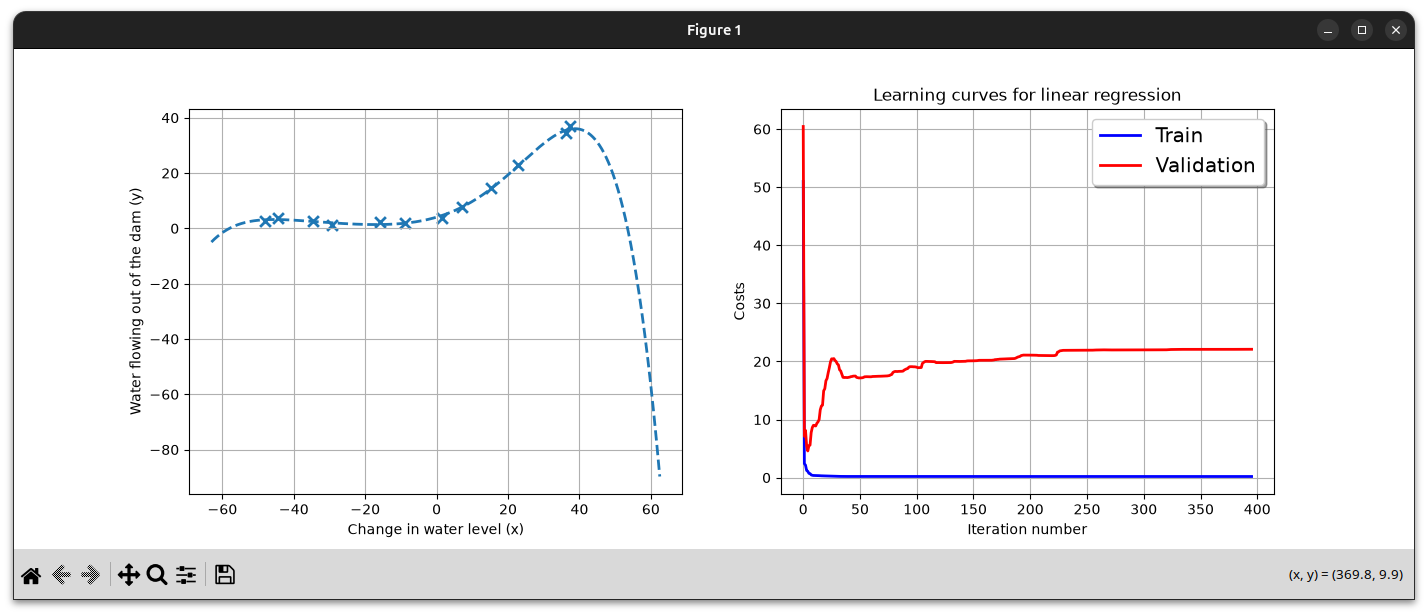
\includegraphics[width=0.75\linewidth]{figure/image7.png}
    \label{fig:placeholder}
\end{figure}

The polynomial model fits the training data well, but the curve changes too much at the extremes.

The training cost is very low, while the validation cost remains high.

This indicates overfitting (high variance) because the model does not perform well on new data.

\subsection{| 5.2 Adjusting the regularization hyper-parameter}

\begin{figure}[H]
    \centering
    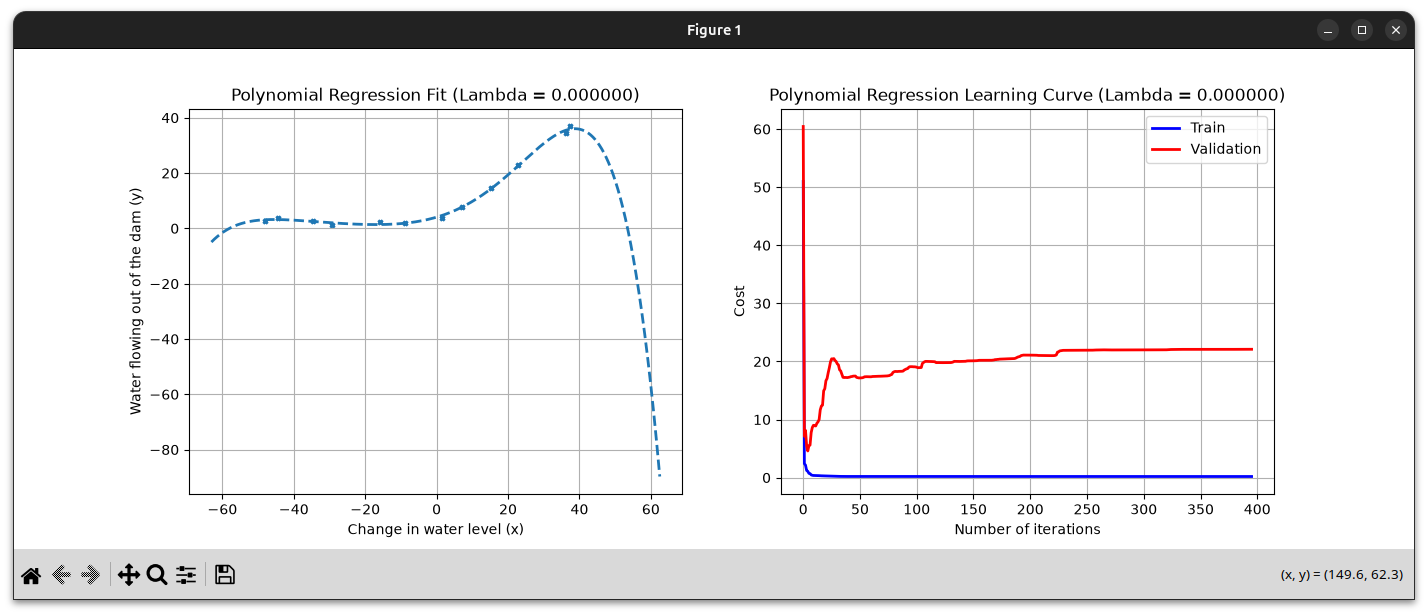
\includegraphics[width=0.75\linewidth]{figure/image8.png}
    \label{fig:placeholder}
\end{figure}

\begin{figure}[H]
    \centering
    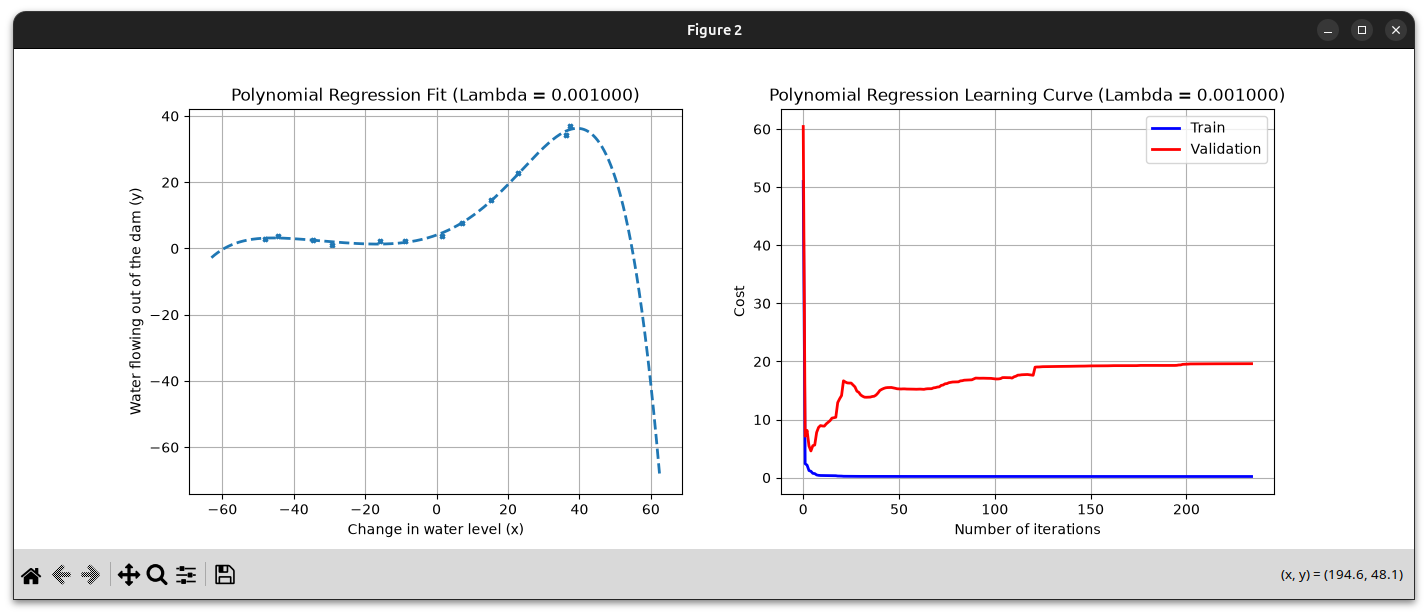
\includegraphics[width=0.75\linewidth]{figure/image9.png}
    \label{fig:placeholder}
\end{figure}

\begin{figure}[H]
    \centering
    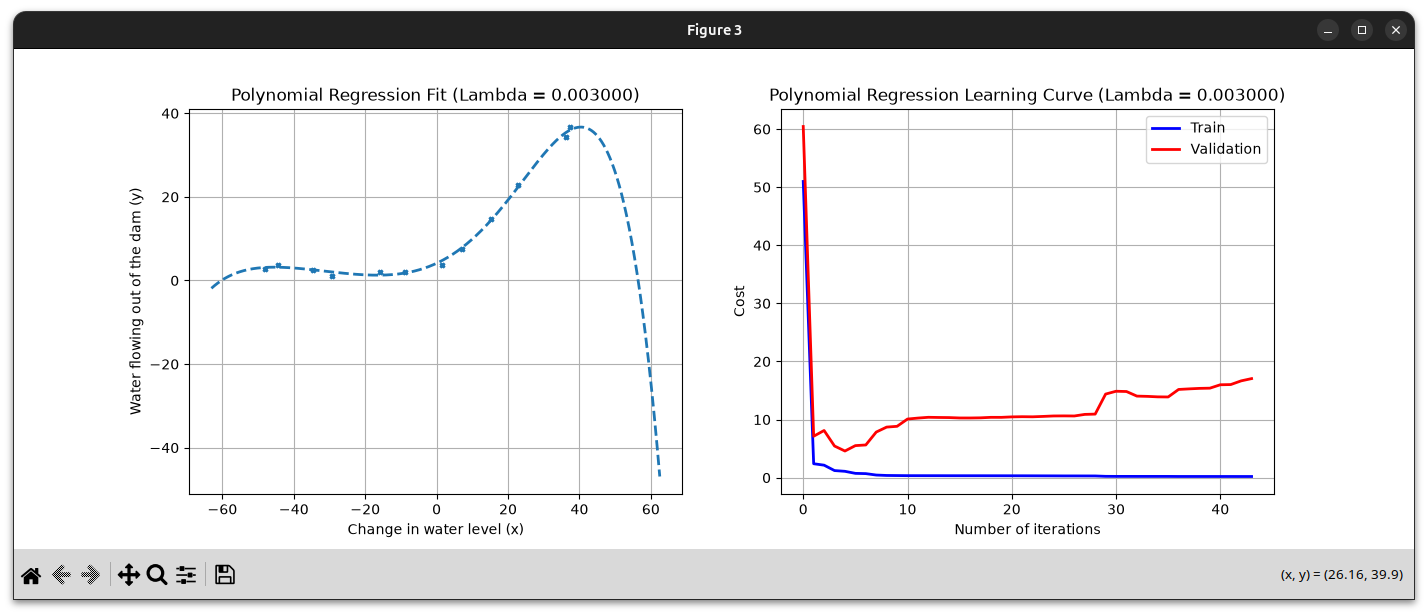
\includegraphics[width=0.75\linewidth]{figure/image10.png}
    \label{fig:placeholder}
\end{figure}

\begin{figure}[H]
    \centering
    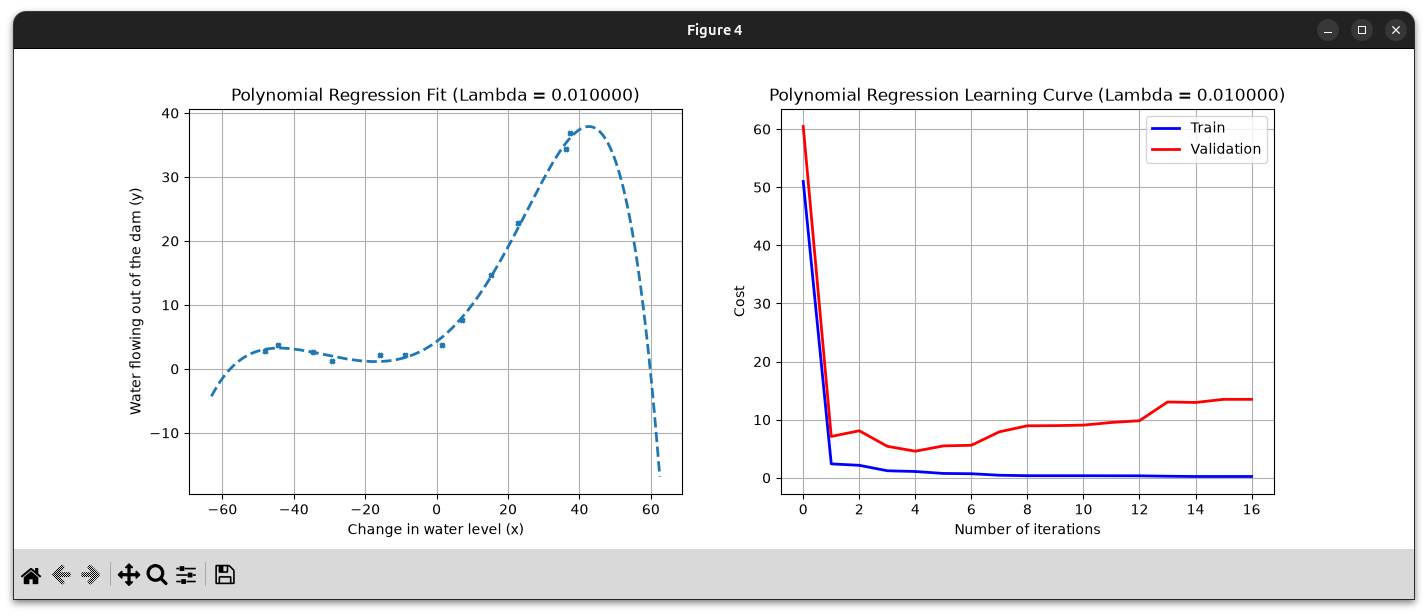
\includegraphics[width=0.75\linewidth]{figure/image11.png}
    \label{fig:placeholder}
\end{figure}

\begin{figure}[H]
    \centering
    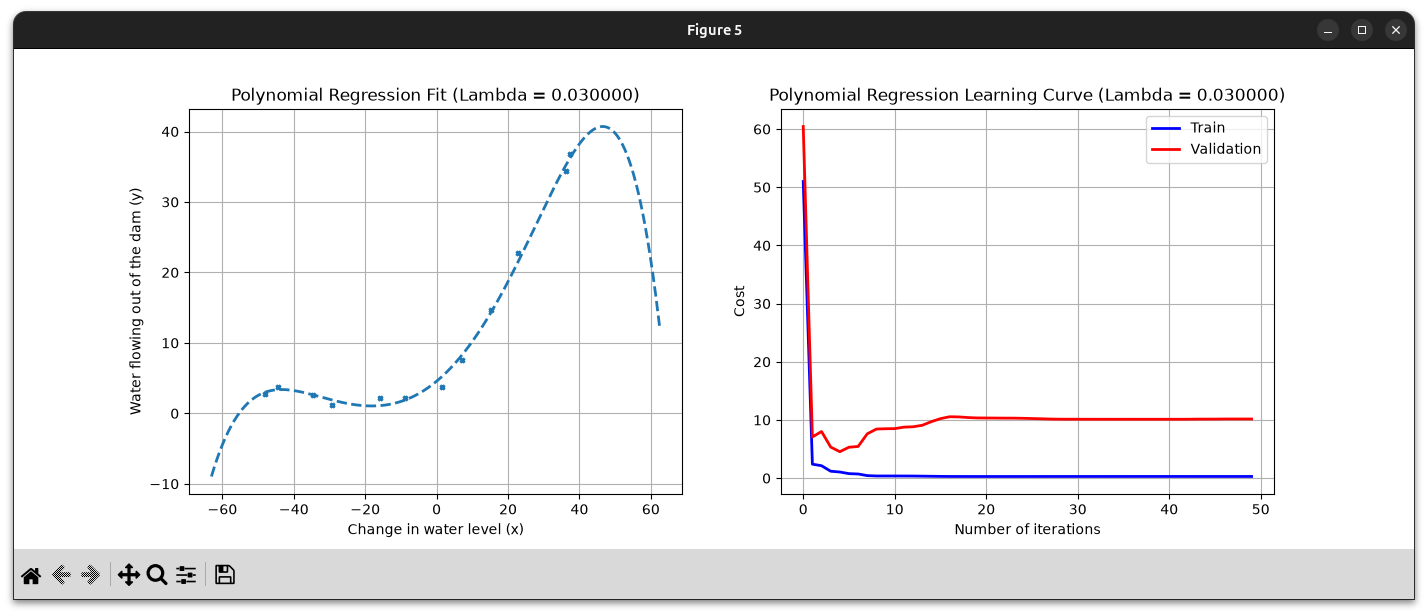
\includegraphics[width=0.75\linewidth]{figure/image12.png}
    \label{fig:placeholder}
\end{figure}

\begin{figure}[H]
    \centering
    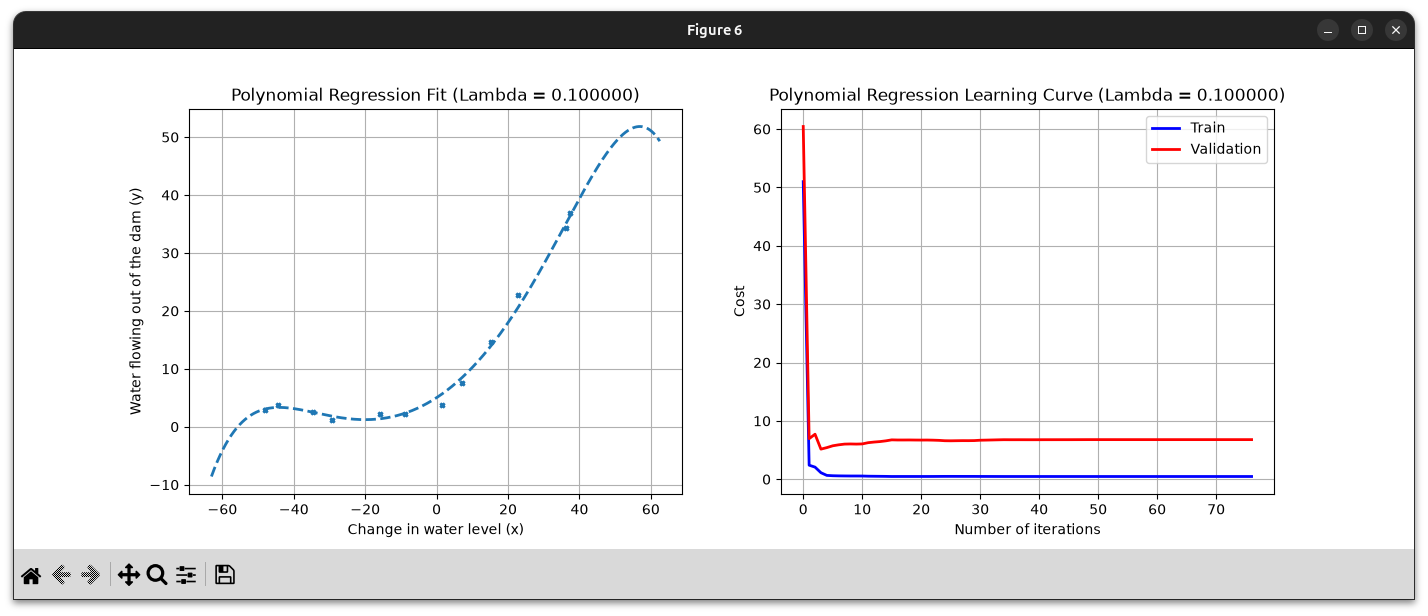
\includegraphics[width=0.75\linewidth]{figure/image13.png}
    \label{fig:placeholder}
\end{figure}

\begin{figure}[H]
    \centering
    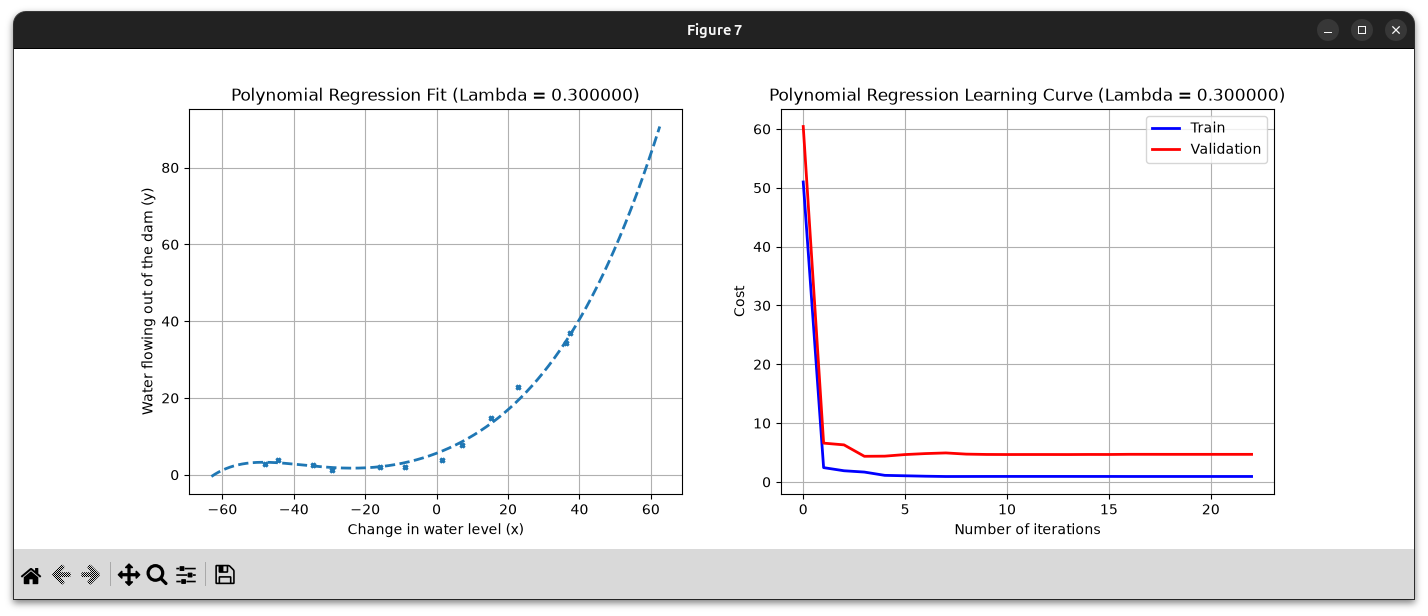
\includegraphics[width=0.75\linewidth]{figure/image14.png}
    \label{fig:placeholder}
\end{figure}

\begin{figure}[H]
    \centering
    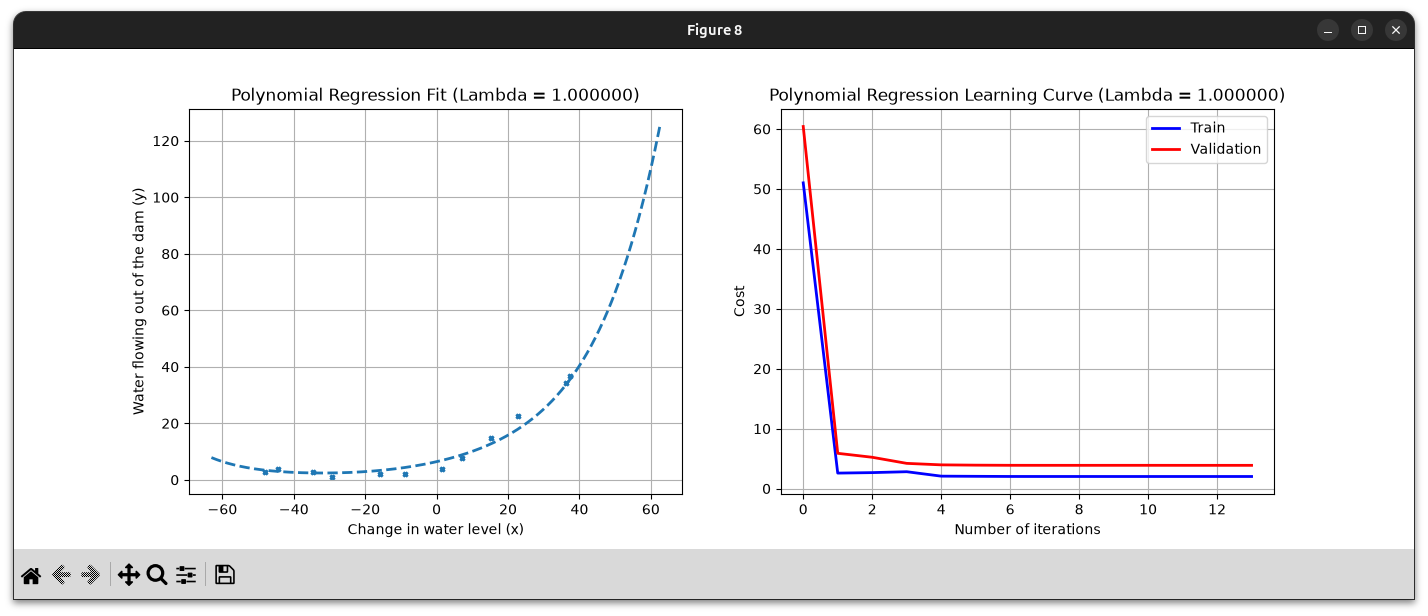
\includegraphics[width=0.75\linewidth]{figure/image15.png}
    \label{fig:placeholder}
\end{figure}

\begin{figure}[H]
    \centering
    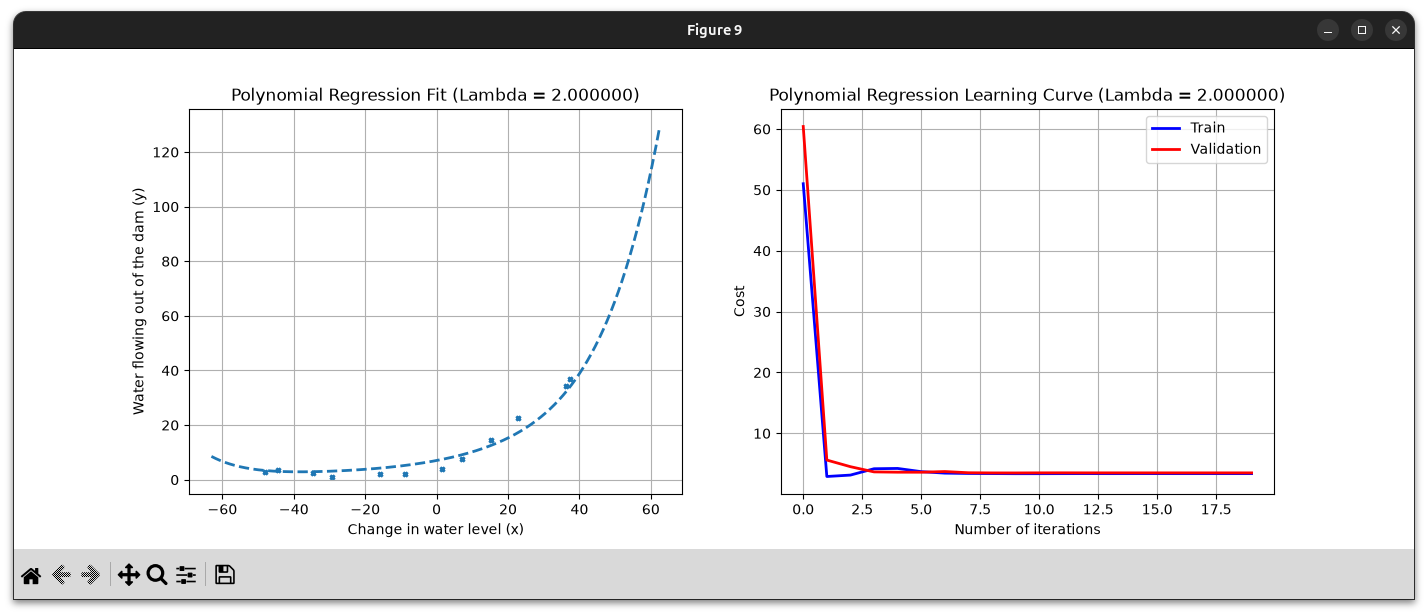
\includegraphics[width=0.75\linewidth]{figure/image16.png}
    \label{fig:placeholder}
\end{figure}

\begin{figure}[H]
    \centering
    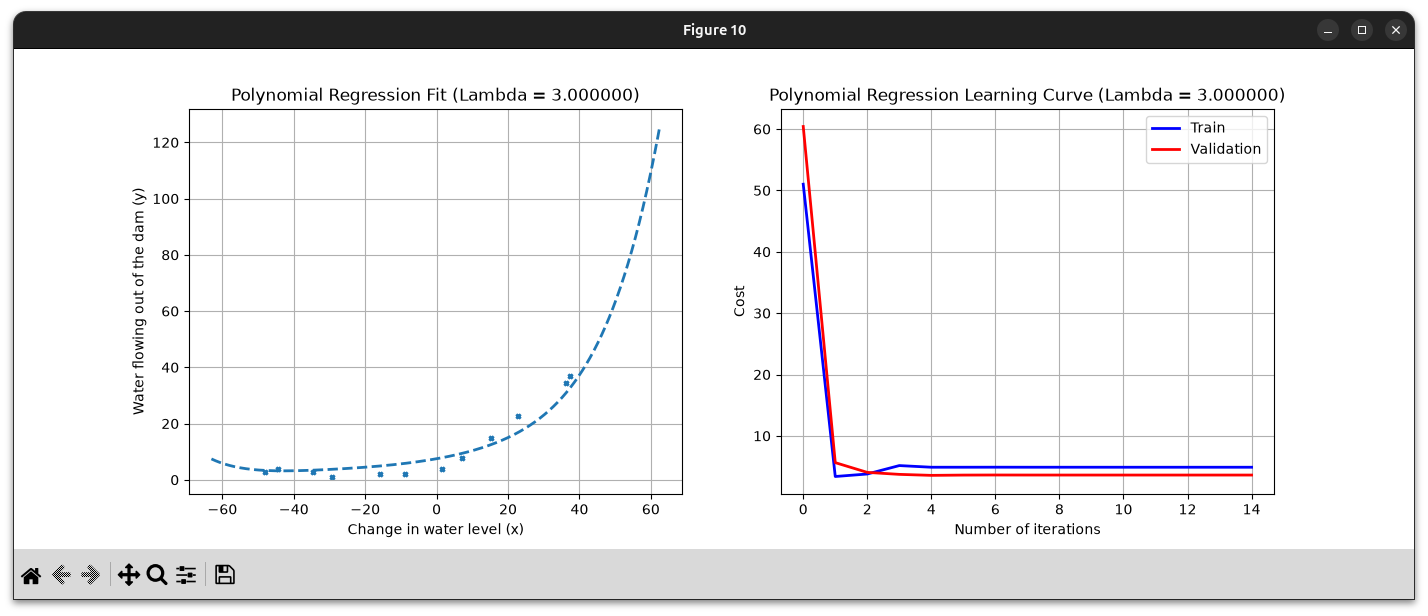
\includegraphics[width=0.75\linewidth]{figure/image17.png}
    \label{fig:placeholder}
\end{figure}

\begin{figure}[H]
    \centering
    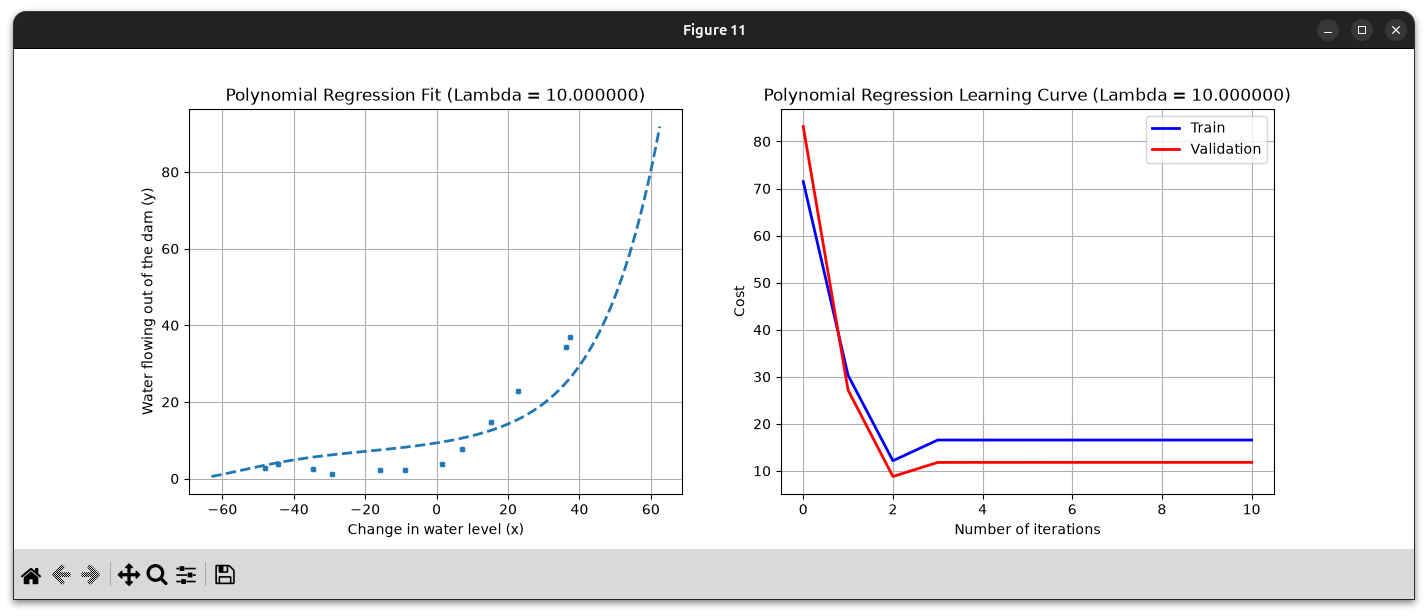
\includegraphics[width=0.75\linewidth]{figure/image18.png}
    \label{fig:placeholder}
\end{figure}

\begin{figure}[H]
    \centering
    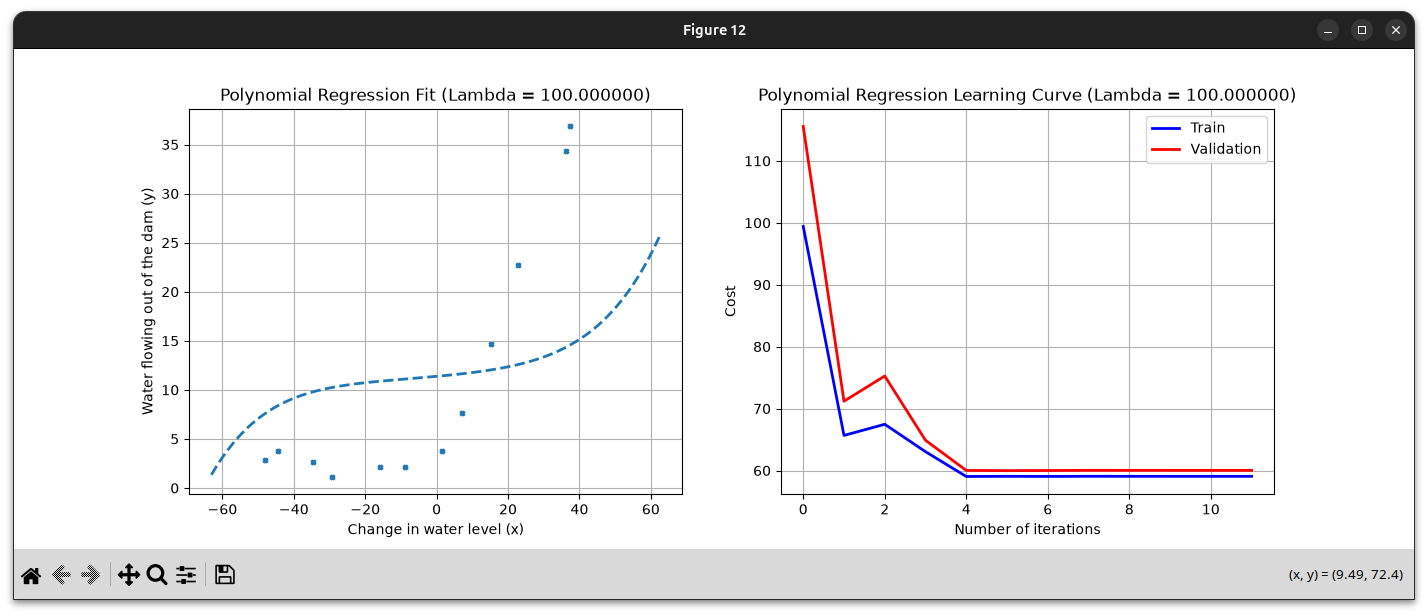
\includegraphics[width=0.75\linewidth]{figure/image19.png}
    \label{fig:placeholder}
\end{figure}



When \(\lambda=0\), the model fits the training data very well, but the validation cost is high. This indicates overfitting (high variance).

When \(\lambda=1\), the model fits the data well, and both costs are relatively low.

When \(\lambda=100\), the regularization is too strong, and both costs are high. This indicates underfitting (high bias).

Increasing \(\lambda\) reduces overfitting, but too much regularization causes underfitting.

\subsection{| 5.3 Selecting $\lambda$ using a validation set}

\begin{figure}[H]
    \centering
    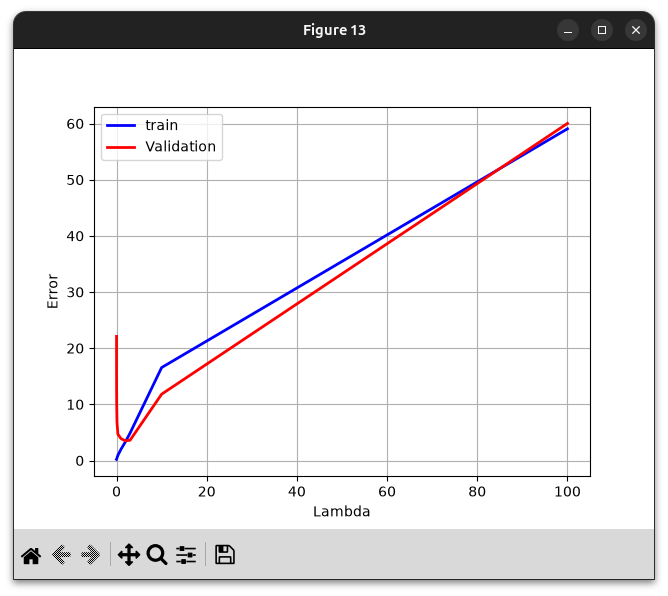
\includegraphics[width=0.75\linewidth]{figure/image20.png}
    \label{fig:placeholder}
\end{figure}

The validation cost is high when \(\lambda=0\), indicating overfitting.

As \(\lambda\) increases, the validation cost decreases. However, when \(\lambda\) is too high, both costs increase, indicating underfitting.

The best \(\lambda\) is the one with the lowest validation cost.

\begin{lstlisting}
# =========== Part:  Computing test set error =============
Lambda = 2.0 # change to Lambda to the best value
\end{lstlisting}

\subsection{| 5.4 Computing test set error}


\begin{figure}[H]
    \centering
    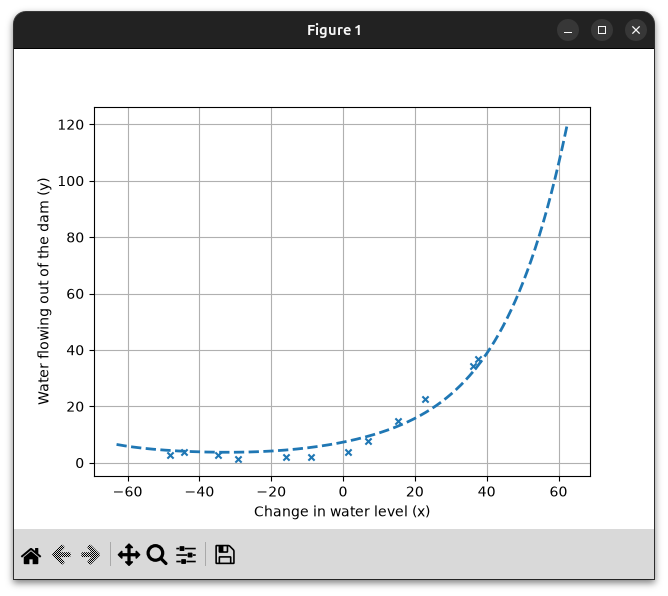
\includegraphics[width=0.75\linewidth]{figure/image21.png}
    \label{fig:placeholder}
\end{figure}

\begin{figure}[H]
    \centering
    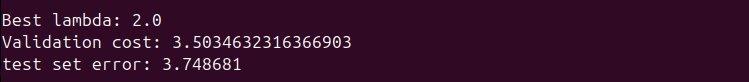
\includegraphics[width=0.75\linewidth]{figure/image22.png}
    \label{fig:placeholder}
\end{figure}

The best value of \(\lambda\) is 2, with a validation cost of 3.5035.

The test cost is 3.7487, which is close to the validation cost.

This shows that the model fits the data well and gives good results on new data.

\subsection{| 5.5 Some questions, you have to answer...}

· Comment découpe-t-on un jeu de données pour entraîner et évaluer un modèle de prédiction?
\vspace{\baselineskip}

R: On peut diviser les données en trois parties : les données d'entraînement (training set), de validation (validation set) et de test (test set).
\vspace{\baselineskip}

· Définissez ce qu’est la capacité d’un modèle de prédiction (i.e. sa complexité). Sur quel ensemble
l’évalue-t-on?
\vspace{\baselineskip}

R: C'est la capacité du modèle à représenter les tendances des données, qu'elles soient simples ou complexes. On peut évaluer son ajustement avec les données d'entraînement.

· Définissez le concept d’erreur de généralisation? Sur quel ensemble l’évalue-t-on?
\vspace{\baselineskip}

R: C'est l'erreur du modèle lorsqu'il fait des prédictions sur de nouvelles données. On l'évalue avec les données de test.
\vspace{\baselineskip}

· A quoi sert l’ensemble de validation?
\vspace{\baselineskip}

R: Il sert à comparer les résultats du modèle avec différents hyperparamètres, comme lambda, pour choisir celui qui donne la plus petite erreur de validation.
\vspace{\baselineskip}

· Comment trouver les paramètres et fixer les hyperparamètres?
\vspace{\baselineskip}

R: Les paramètres, comme theta, sont calculés pendant l'entraînement en minimisant la fonction de coût. Les hyperparamètres, comme lambda, sont choisis à partir des résultats de validation.
\vspace{\baselineskip}

· A quoi sert la “learning curve”?
\vspace{\baselineskip}

R: Elle sert à visualiser l'évolution des erreurs d'entraînement et de validation. Elle permet aussi d'identifier les problèmes d'underfitting et d'overfitting.

